\section{Data}

The MNIST dataset is corpus of handwritten digits that is commonly used for training and bench-marking computer vision algorithms. While most models achieve very high accuracy on MNIST, their performance does not generalize well to other datasets. This is because MNIST's simplicity often fails to effectively represent model performance on modern computer vision tasks (i.e. detection, segmentation) \cite{xiao2017/online}. Thus, in this project, we use the Fashion-MNIST dataset produced by e-commerce company Zalando to alleviate some of the common issues stemming from the traditional MNIST dataset. 

The Fashion-MNIST dataset consists of 70,000 28x28 grayscale images. 60,000 of these images belong to the training set, while the remaining 10,000 belong to the test set. There are 10 labels, with integer labels of 0-9 as follows: \{T-shirts/top, Trouser, Pullover, Dress, Coat, Sandal, Shirt, Sneaker, Bag, Ankle boot\}. Hence, the data type is nominal discrete. This dataset is highly heterogeneous yet also extensive, making it a highly promising for studying classification with BCNNs.

We use Uniform Manifold Approximation and Projection (UMAP) \cite{mcinnes2018umap-software} to project and visualize our raw data. This embedding method is a successor to t-Distributed Stochastic Neighbor Embedding (t-SNE). UMAP uses graph layout algorithms to arrange data in low-dimensional space. The algorithm constructs a high dimensional graph representation of our data – called a fuzzy simplicial complex – and then optimizes the low-dimensional graph to be as structurally similar as possible. This is advantageous because while t-SNE does not preserve global data structure, UMAP's inter-cluster distances are just as interpretable as intra-cluster distances. Thus, UMAP ensures that local structure is preserved in balance with global structure. 

Our projection separates the classes while preserving the global structure (Figure~\ref{fig:Fashion_MNIST_UMAP}). In general, the projection separated pants and footwear from shirts, coats and dresses, which are significantly different types of clothing. Unlike easier datasets (i.e. MNIST), there were classes that did not separate cleanly. Specifically, T-shirts, shirts, dresses, pullovers, and coats overlap in the 2D projection. More ideal separation can be realized by using label information with UMAP; however, the goal is to predict classes without labels.

\begin{figure}[t]
  \centering
  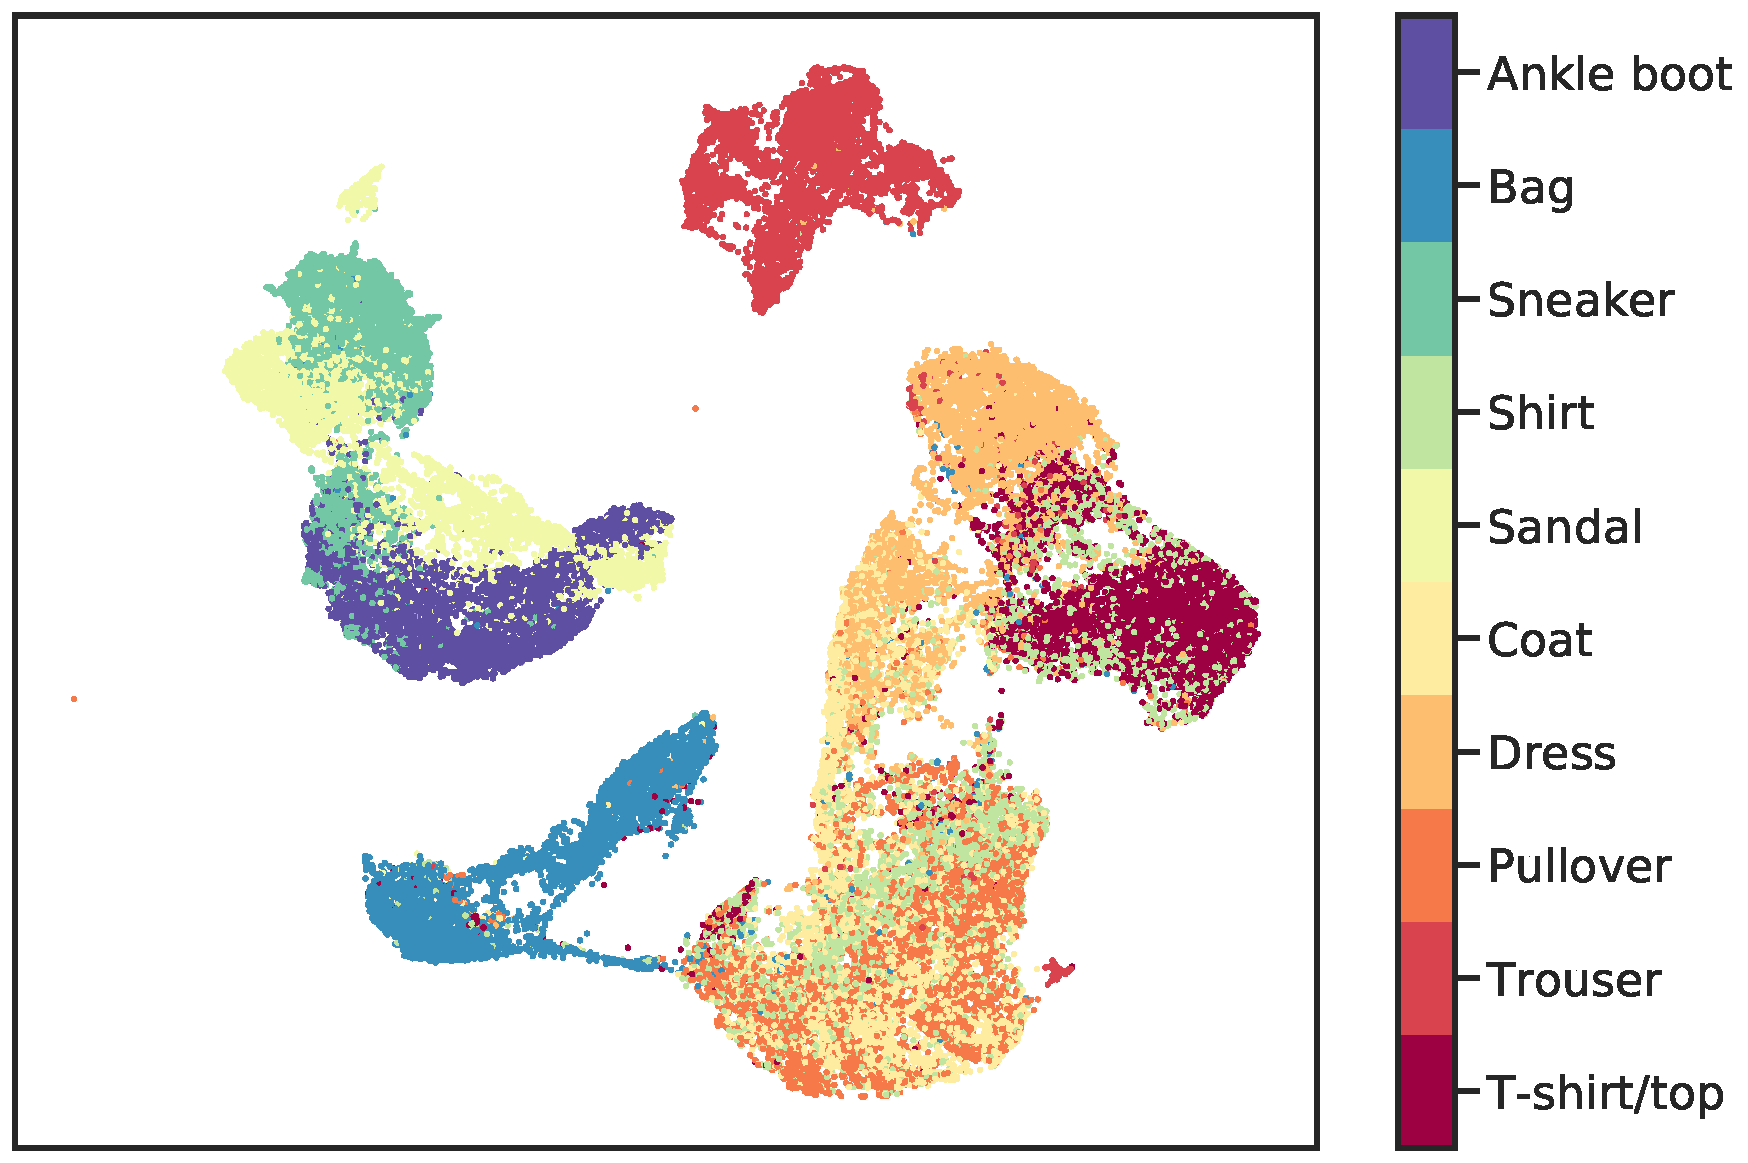
\includegraphics[width=\columnwidth]{Figures/Fashion_MNIST_UMAP.pdf}
  \caption{UMAP Projection of Fashion MNIST data Based on RAW Pixel Values}
%   \vspace{-1.5em}
  \label{fig:Fashion_MNIST_UMAP}
  \vspace{-1em}
\end{figure}